\graphicspath{{../Graphics/Cpt2-InjectCW/}}

Una forma alternativa de obtención de OFC es mediante la inyección de luz láser en otro láser de semiconductor funcionando en corriente constante. Sin embargo este sistema presenta una dinámica no lineal muy variada aparte de la observación de los OFC. En este cápitulo se han estudiado los distintos comportamientos no lineales observados en este sistema en función de las condiciones de la inyección óptica, dadas por la potencia inyectada $P_{Iny}$ y la diferencia de frecuencias $\delta \nu$ entre el láser maestro y el láser esclavo (ML y SL respectivamente por sus siglas en inglés). Se ha trabajado con el láser SL en corriente continua con $\ibias = 35$ mA, $V_{RF} = 0$ V y $f_R = 5.0$ GHz.

Se han obtenido los diferentes régimenes dinámicos de SL en función de $P_{Iny}$ para dos valores de $\delta\nu$ distintos, uno positivo que equivale a una frecuencia de SL menor que la de ML, y otro negativo con el caso contrario.

En la Figura \ref{Img:zonasIO} se muestran los espectros ópticos del láser esclavo con inyecci\'on \'optica de las diferentes regiones dinámicas obtenidas para diferentes valores de $P_{Iny}$ a $\delta\nu = -2$ GHz. 

			\begin{figure}[H]
				\centering
				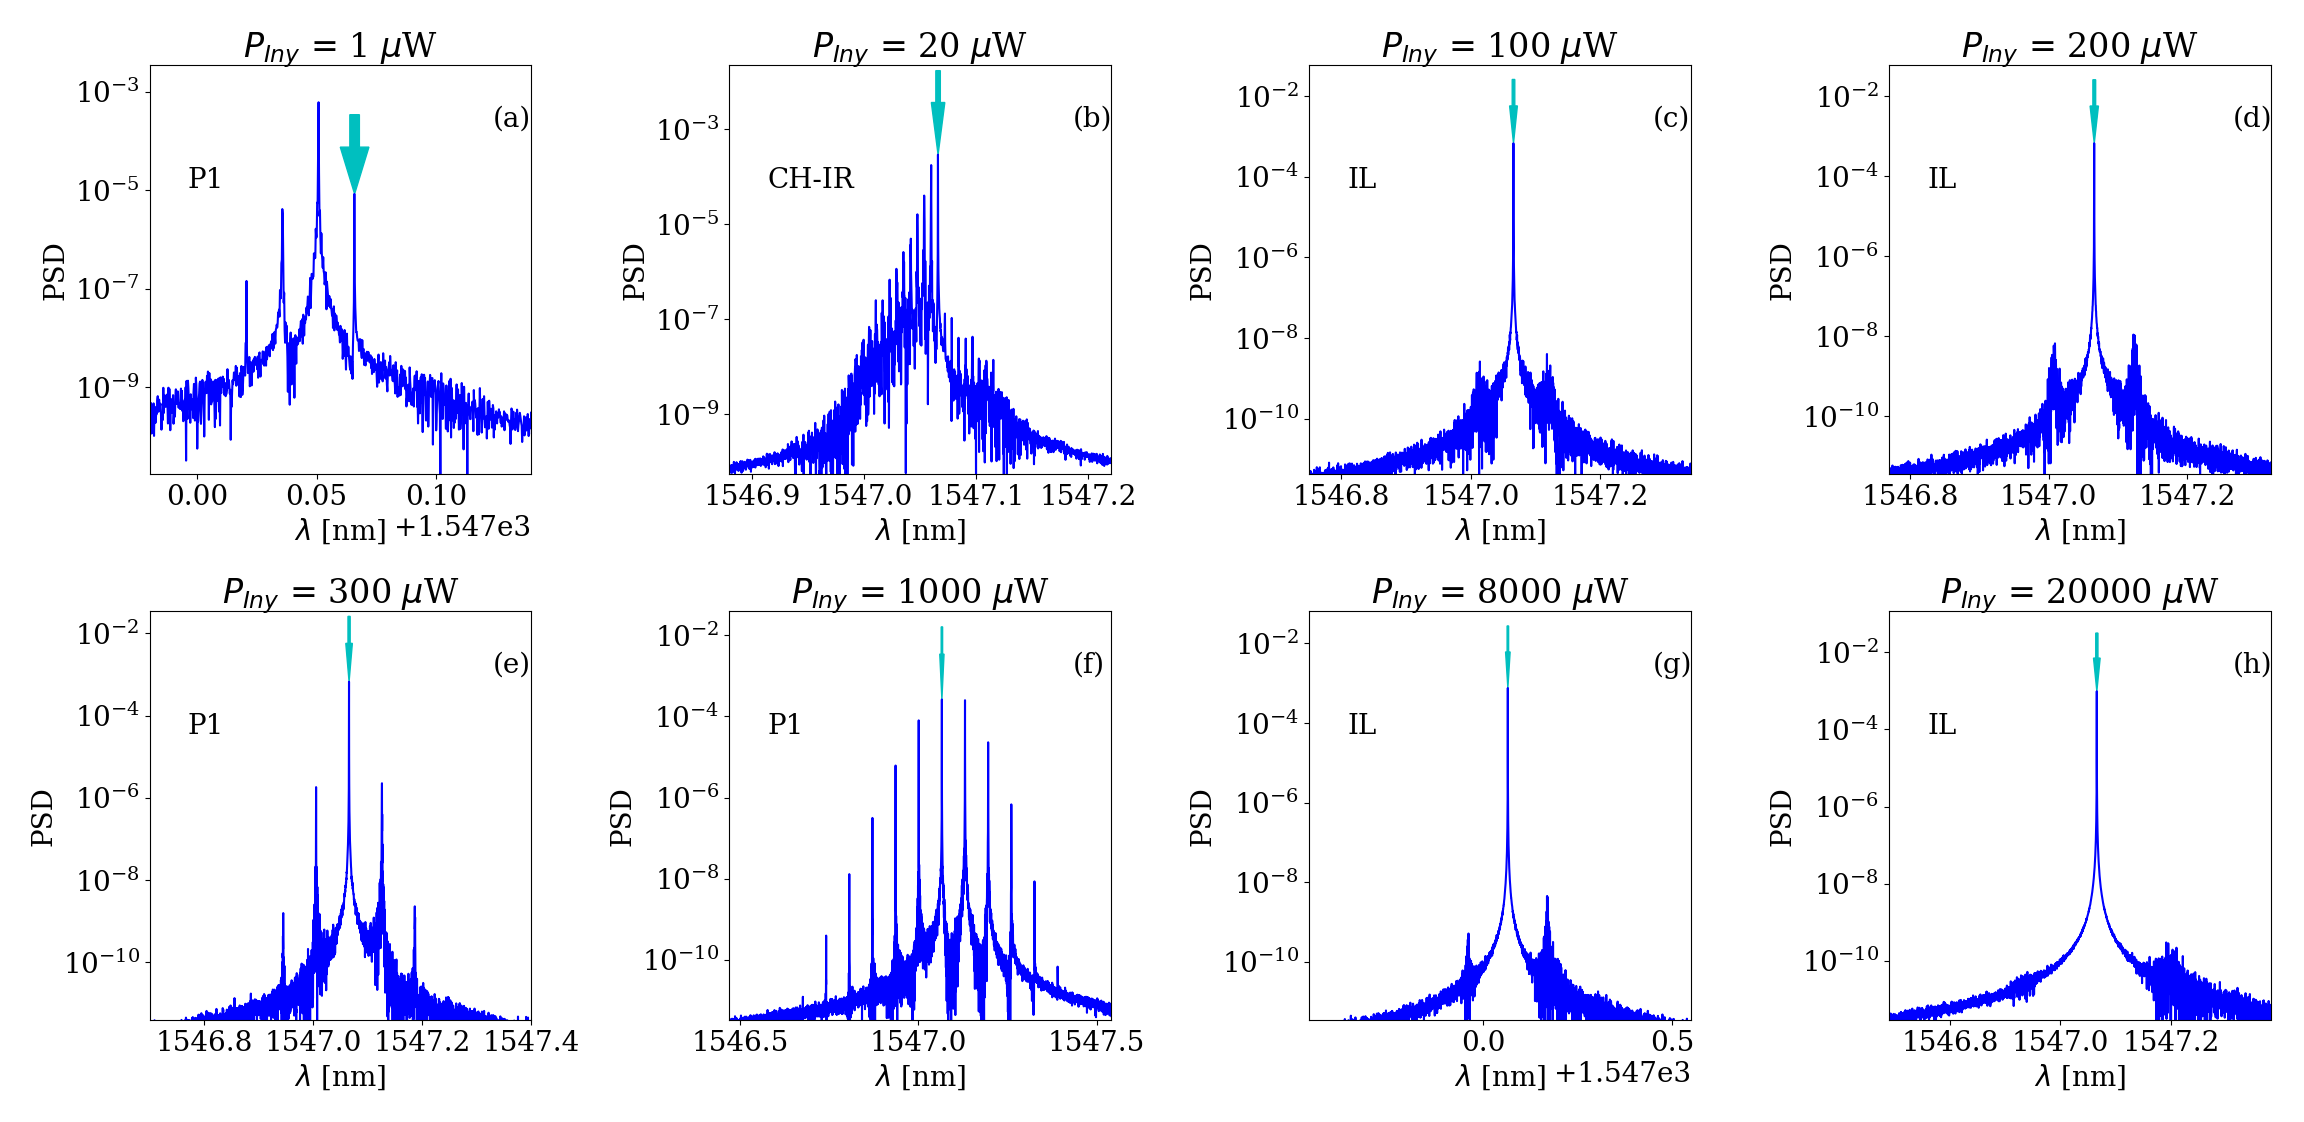
\includegraphics[width=1.0\linewidth]{zoneMap.png}
				\caption{\label{Img:zonasIO}Espectros ópticos con inyección \'optica de las diferentes regiones dinámicas obtenidas para diferentes valores de $P_{Iny}$ para $\delta\nu = -2$ GHz. Se indica la frecuencia de inyección $\nu_{ML}$ con una flecha y $P_{Iny}$ para cada espectro óptico.}
			\end{figure}

Para una baja potencia de inyección $P_{Iny} = 1 \; \mu$W (Figura \ref{Img:zonasIO} (a)) se obtiene un espectro óptico con el pico de emisión de SL y tres picos satélites, uno de ellos apareciendo a $\nu_{ML}$ y los otros simétricos respecto al pico principal. En esta región denominada de periodo 1, P1, las variables internas del láser tienen un comportamiento periodico. Cuando las potencias de inyección son bajas, la frecuencia de este comportamiento es $\delta\nu$ debido a un fenómeno de \textit{Four-wave mixing} (FWM, mezcla de cuatro ondas) \cite{van1995semiconductor}. Al aumentar $P_{Iny}$ se llega a una región de caos, CH-IR ($P_{Iny} = 20\; \mu$W, Figura \ref{Img:zonasIO} (b)), con un OFC formado por muchas líneas y con un perfil irregular. Esta región de caos se destruye para $P_{Iny} = 100\;\mu$W, en la que se obtiene un espectro óptico con una única línea de emisión para la frecuencia de inyección $\nu_{ML}$. Al aumentar la potencia de ML el láser deja de emitir en $\nu_{SL}$ pasando a emitir solo en $\nu_{ML}$. A este fenómeno se le conoce como Bloqueo de Inyección (IL por sus siglas en inglés). El régimen IL se caracteriza además porque el láser esclavo pasa a emitir con una fase óptica relativa a la del láser maestro con un valor constante. Además la potencia del láser esclavo es constante. En la Figura \ref{Img:zonasIO} (d) se muestra el espectro para $P_{Iny} = 200\;\mu$W en IL, observando como al aumentar la potencia de inyección se empiezan a excitar los picos satélites correspondientes a las oscilaciones de relajación. Esto indica que nos encontramos en el límite de dos comportamientos, el descrito para la región IL y un comportamiento periódico, con periodo el de las oscilaciones de relajación. Este cambio de comportamientos corresponde a una bifurcación de Hopf. Si se continúa aumentando la potencia de inyección aumentarán los picos de la frecuencia de oscilaciones de relajación, retornando a la región P1 ($V_{RF} = 300\;\mu$W, Figura \ref{Img:zonasIO} (e)). Dentro de la región P1, el aumento de la potencia de inyección produce la aparición de nuevas líneas de emisión, comenzando a aparecer el OFC. A medida que aumenta la potencia de inyección la separación entre líneas consecutivas del espectro óptico va decreciendo, disminuyendo la frecuencia \'optica de separación entre l\'ineas $\Delta f$. Para $P_{Iny} = 300\;\mu$W se tiene $\Delta f = 5$ GHz y para $P_{Iny} = 1000\;\mu$W se tiene $\Delta f = 4.6$ GHz. Para altas potencias de inyección, $P_{Iny} = 8000 \;\mu$W y $20000 \;\mu$W, se regresa a la región IL.

		A partir de los datos experimentales para un láser de modo discreto en corriente continua $\ibias = 30$ mA \cite{Chaves19}, se ha obtenido un mapa con las diferentes regiones dinámicas en función de la potencia inyectada experimental $P_{Inj}$ y $\delta\nu$. Hacemos notar que la potencia inyectada teórica $P_{Iny}$ es siempre mayor que la potencia inyectada experimental $P_{Inj}$ debido a las pérdidas que sufre la luz del láser maestro en el experimento antes de ser inyectado en el láser esclavo. Se ha estimado el término de proporcionalidad entre ambas potencias de la siguiente forma. Se ha observado que al aumentar $P_{Inj}$, el comportamiento IL se empieza a obtener experimentalmente en $P_{Inj} = 6\;\mu$W \cite{Chaves19}. Como en las simulaciones ese comportamiento se empieza a observar en $P_{Iny} = 77.9\;\mu$W, estimamos que $P_{Inj} = 0.077 \cdot P_{Iny}$. Aunque la corriente teórica es diferente de la experimental la comparación es adecuada porque en ambos casos la relación entre la corriente y la corriente umbral es similar $\frac{\ibias}{I_{th}} \approx 2.3$. En la Figura \ref{fig:map} se muestra el mapa de las regiones dinámicas obtenido a partir de \cite{Chaves19}, marcando los puntos correspondientes a los espectros ópticos de la Figura \ref{Img:zonasIO}.

			\begin{figure}[H]
				\centering
				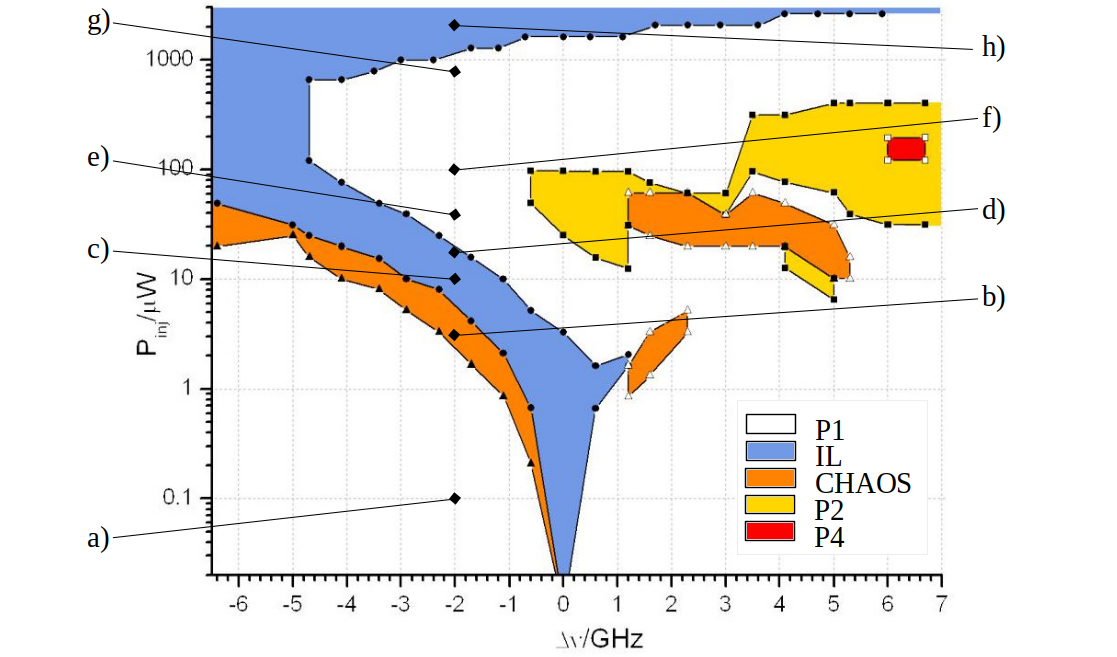
\includegraphics[width=0.7\linewidth]{maps.png}
				\caption{\label{fig:map}Mapa con las diferentes regiones dinámicas en función de $P_{Inj}$ y $\delta\nu$ obtenido a partir de \cite{Chaves19}. Se han marcando los puntos correspondientes a los espectros ópticos de la Figura \ref{Img:zonasIO}.}
			\end{figure}

		Las regiones dinámicas del mapa de la Figura \ref{fig:map} obtenidas experimentalmente, para las condiciones de inyección de los espectros ópticos de la Figura \ref{Img:zonasIO} corresponden a las regiones obtenidas del análisis de los resultados de la simulación. Lo cuál, indica un buen acuerdo entre teoría y experimento.

		En la Figura \ref{fig:zoneRtEq} se muestran la potencia $P(t)$, la fase óptica $\Phi (t)$ y el espectro óptico de los tres casos más representativos de la Figura \ref{Img:zonasIO} para cada región dinámica obtenida: CH-IR, IL y P1. Esto permite estudiar los procesos que tienen lugar en las tres regiones encontradas para $\delta\nu = -2$ GHz. Se hace notar que la fase que dibujamos en esta figura es $\Phi - 2\pi\delta\nu't$, donde $\Phi$ es la obtenida en la ecuación \ref{eq:RtEq-Ph}. Esta $\Phi$ está referida a la frecuencia del láser en el umbral. Así la fase dibujada es la referida a la frecuencia de la inyección óptica $\nu_{ML}$ en vez de a la frecuencia en el umbral $\nu_{th}$. 

			\begin{figure}[H]
				\centering
				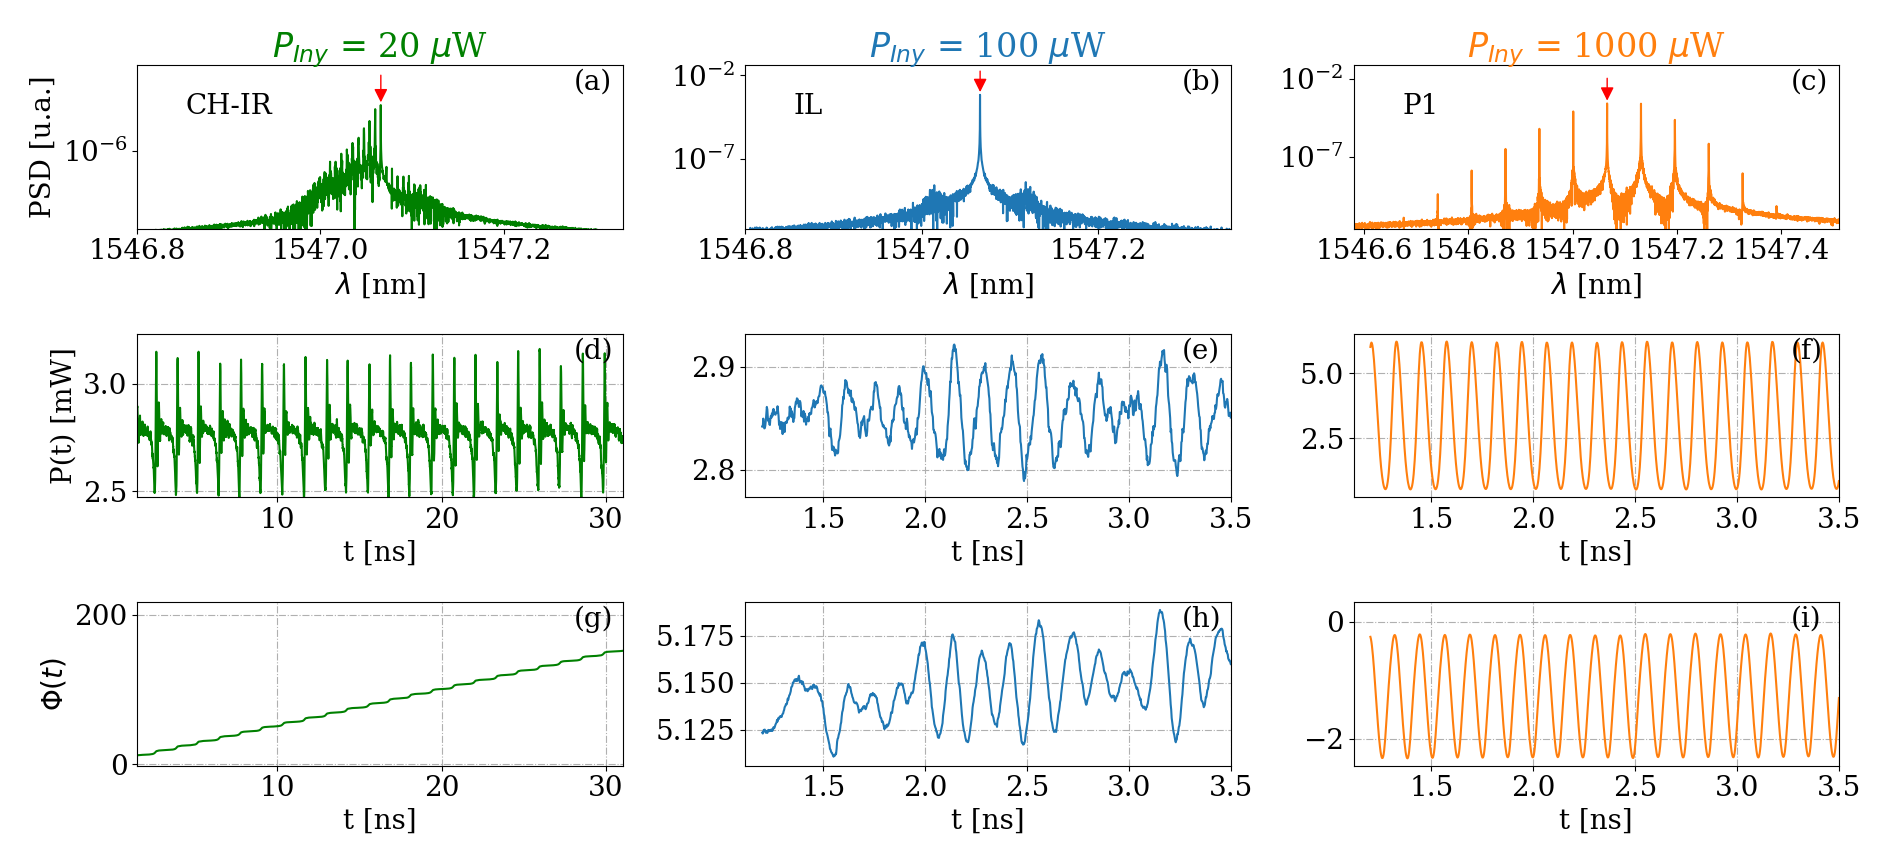
\includegraphics[width=1.0\linewidth]{zoneRtEq.png}
				\caption{\label{fig:zoneRtEq}Potencia $P(t)$, fase óptica $\Phi (t)$ y espectro óptico de los tres casos más representativos de la Figura \ref{Img:zonasIO} para cada región dinámica obtenida: CH-IR con $P_{Iny} = 20\;\mu$W (verde), IL con $P_{Iny} = 100\;\mu$W (azul) y P1 con $P_{Iny} = 1000\;\mu$W (naranja). Se indica en los espectros la frecuencia de inyección $\nu_{ML}$ con una flecha.}	
			\end{figure}

		Para el caso con $P_{Iny} = 1000\;\mu$W de la región P1 se obtiene en el espectro óptico (Figura \ref{fig:zoneRtEq} (c)) OFC de buena calidad formado por varias líneas bien resueltas y con las misma separación entre ellas ($\Delta f = 4.6$ GHz). Los perfiles temporales que se obtienen para $P(t)$ y $\Phi(t)$ son oscilaciones con una amplitud y una frecuencia bien definidos con $\Delta f = 4.6$ GHz. En la Figura \ref{fig:zoneRtEq} (e)  se muestra el perfil temporal de la potencia para $P_{Iny} = 100\;\mu$W IL, que toma un valor aproximadamente constante. Esto mismo se observa para su fase óptica (Figura \ref{fig:zoneRtEq} (h)) en la que se obtienen variaciones de $\Phi(t)$ tres ordenes de magnitud menores que para P1. La representación de $\Phi - 2\pi\delta\nu't$ permite ilustrar mejor este comportamiento constante. Con $P_{Iny} = 20\;\mu$W se encuentra la región CH-IR, obteniendo un espectro irregular. De igual manera se obtienen trazas irregulares para la potencia $P(t)$, con picos irregulares (Figura \ref{fig:zoneRtEq} (d)). Para la fase óptica se observa como va aumentando con saltos de $2\pi$ cada vez que se produce uno de los pulsos irregulares de potencia. En el caso de la fase \'optica se observa como \'esta va aumentando con saltos de $2 \pi$debido a que se trabaja con \'angulos y as\'i estos saltos equivalen al mismo valor. 

		Del mapa de regiones dinámicas de la Figura \ref{fig:map} se deduce que para $\delta\nu$ positivo se ha de poder alcanzar regiones con doblamiento de periodo, P2. En la Figura \ref{fig:P2zone} se muestran los espectros ópticos, $P(t)$ y la proyecci\'on del atractor en el plano ($P(t)$, $N(t)$) del espacio de estados; para $\delta\nu = 5$ GHz y $P_{Iny} = 50\;\mu \textrm{W, } 1000\;\mu\textrm{W y } 200\;\mu$W.

			\begin{figure}[H]
				\centering
				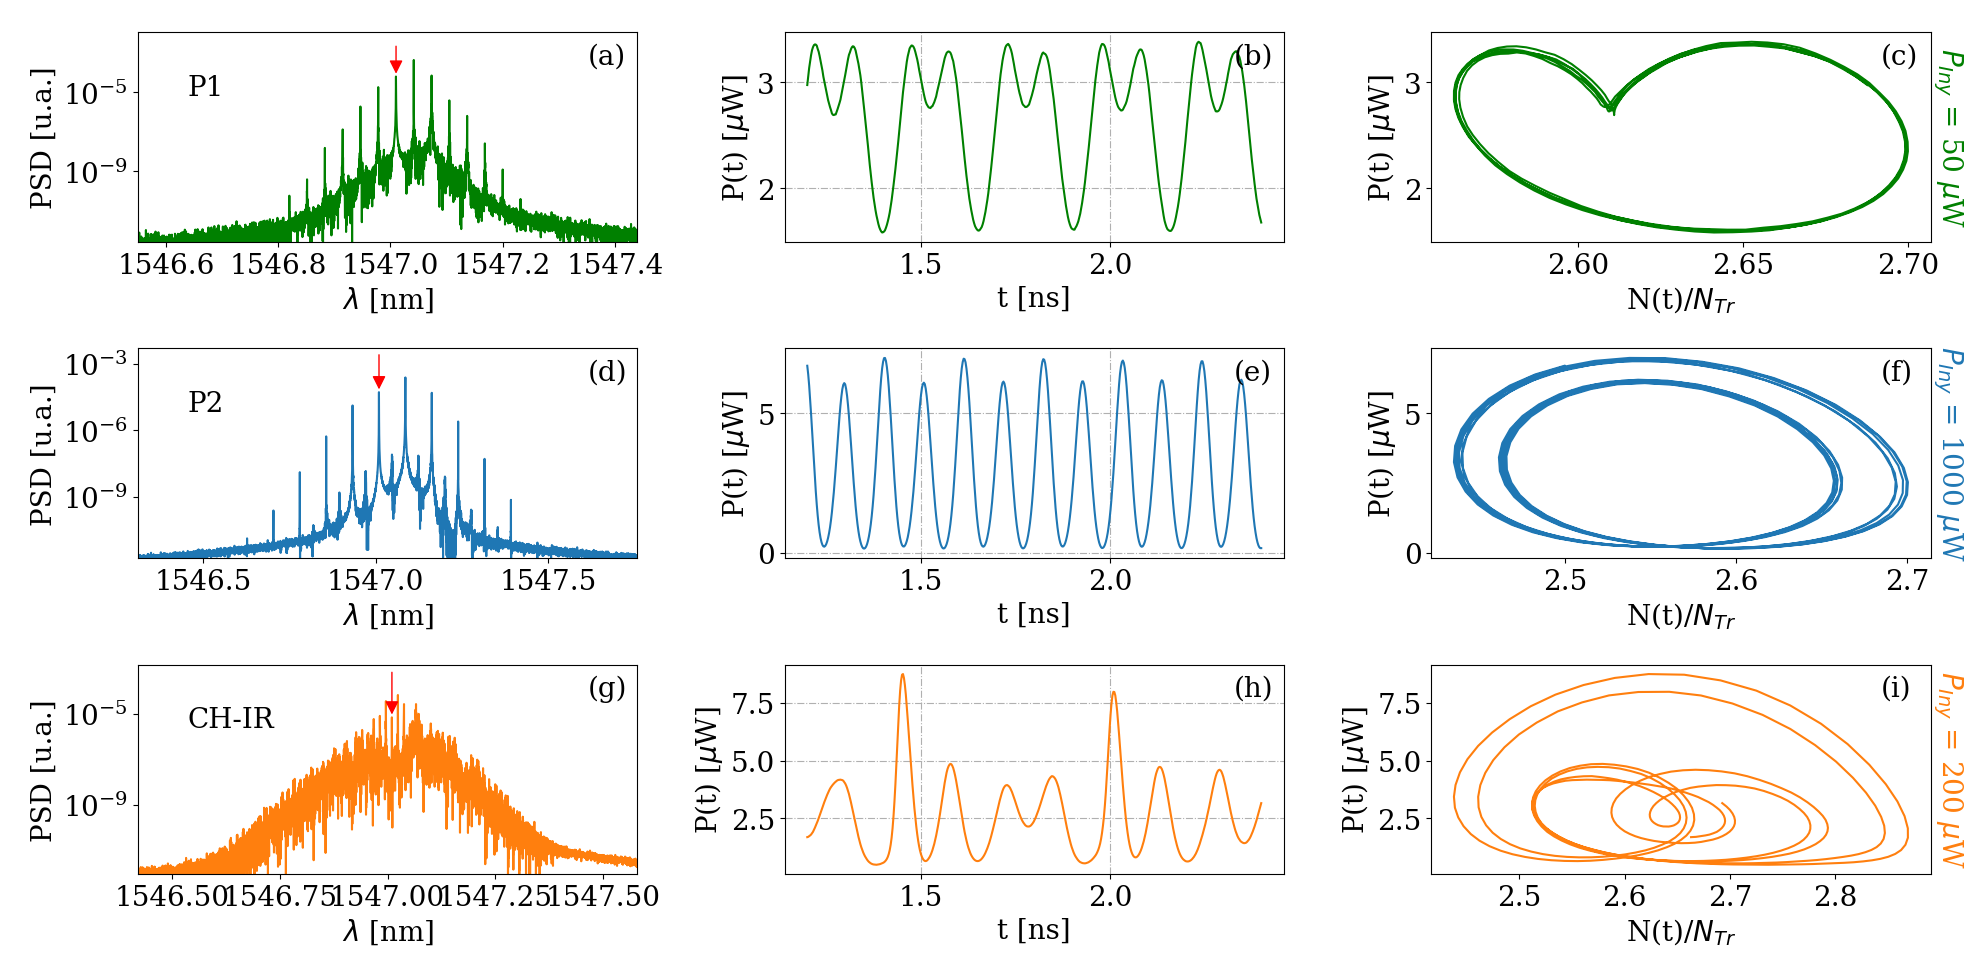
\includegraphics[width=1.0\linewidth]{P2zone.png}
				\caption{\label{fig:P2zone}Espectros ópticos, $P(t)$ y proyecci\'on del atractor en el plano ($P(t)$, $N(t)$) del espacio de estados; para $\delta\nu = 5$ GHz y $P_{Iny} = 50\;\mu \textrm{W (verde), } 1000\;\mu\textrm{W (azul) y } 200\;\mu$W (naranja). Se indica en los espectros la frecuencia de inyección $\nu_{ML}$ con una flecha.}	
			\end{figure}

		Para una diferencia de frecuencias positiva ($\delta \nu = 5$ GHz) y una potencia de inyecci\'on baja de $P_{Iny} = 50\;\mu$W se obtiene un OFC (Figura \ref{fig:P2zone}(a)) de buena calidad con una l\'inea a $\nu_{ML}$ y separaci\'on entre l\'ineas de $\Delta f = 4.2$ GHz ($\Delta \lambda = 0.033$ nm). Para la traza temporal de $P(t)$ (Figura \ref{fig:P2zone} (b)) se obtienen los mismos m\'aximos de potencia para todos los picos. Con una mayor potencia de inyecci\'on ($P_{Iny} = 1000\;\mu$W) se obtiene nuevamente un OFC de gran calidad (Figura \ref{fig:P2zone} (d)), observando unas l\'ineas de emisi\'on dominantes con una separaci\'on entre ellas de $\Delta f = 3.75$ GHz y unas l\'ineas m\'as pequeñas entre las l\'ineas dominantes, cuya separaci\'on entre ellas es tambi\'en $\Delta f = 3.75$ GHz pero cuya separaci\'on con los picos dominantes es la mitad ($\Delta f' = 1.875$ GHz). En el perfil temporal de $P(t)$ de la Figura \ref{fig:P2zone} (e) se observa como se alternan picos con mayor y menor amplitud. Para el caso de las proyecciones del atractor en el plano ($P(t)$, $N(t)$) del espacio de estados se ha obtenido una trayectoria con forma de un \'unico lazo para $P_{Iny} = 50\;\mu$W, mientras que para $P_{Iny} = 1000\;\mu$W la trayectoria describe una curva con autointersección, o doble lazo. Esta diferencia ha llevado a concluir que el caso con $\delta\nu = 5$ GHz y $P_{Iny} = 1000\;\mu$W se encuentra en una regi\'on P2 mientras que para el caso de $\delta\nu = 5$ GHz y $P_{Iny} = 50\;\mu$W se obtiene una regi\'on P1, pues las curvas con doble lazo son características de las soluciones P2 \cite{sconza2005torsion}.

		La región CH-IR se alcanza para $P_{Iny} = 200\;\mu$W, obteniendo un perfil de $P(t)$ con oscilaciones aleatrorias y sin una amplitud o frecuencia determinada (Figura \ref{fig:P2zone} (h)). El OFC del espectro óptico (Figura \ref{fig:P2zone} (g)) se destruye completamente y el diagrama de estados de la Figura \ref{fig:P2zone} (i) describe una trayectoria irregular que para rangos de tiempo suficientemente grandes cubriría todo el espacio. 

		En la Figura \ref{fig:maps2} se muestra el mapa de las regiones dinámicas obtenido en \cite{Chaves19}, marcando los puntos correspondientes a las condiciones de inyección de los resultados de la Figura \ref{fig:P2zone}, obteniendo las mismas regiones que mediante el análisis de los resultados de la simulación.

			\begin{figure}[H]
				\centering
				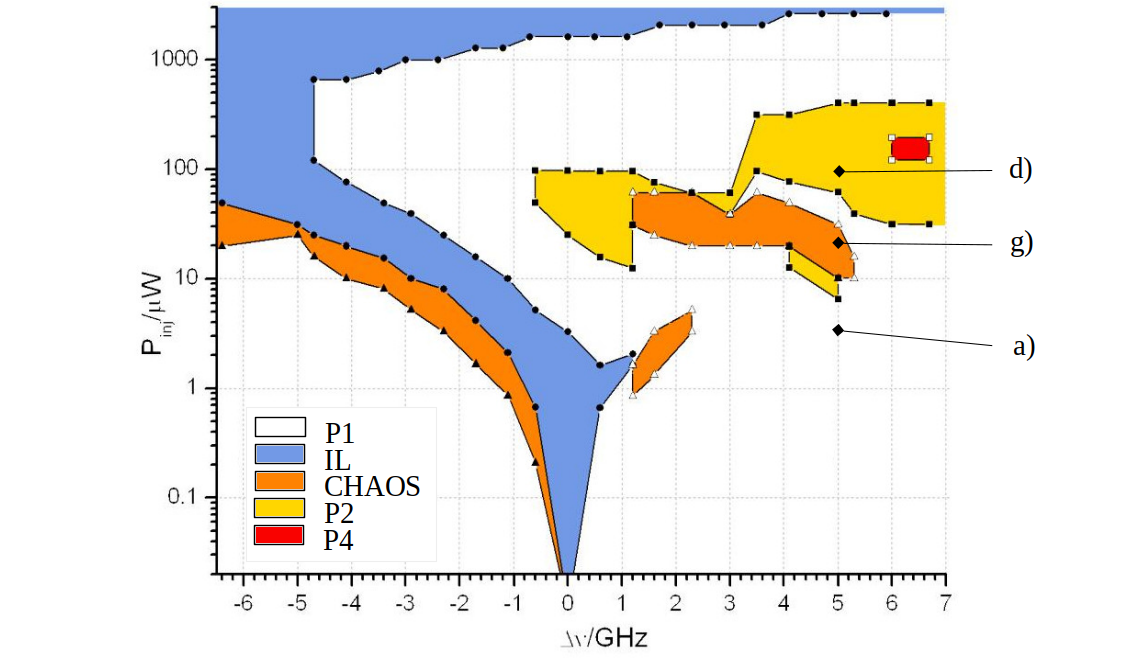
\includegraphics[width=0.7\linewidth]{maps2.png}
				\caption{\label{fig:maps2}Mapa con las diferentes regiones dinámicas en función de $P_{Inj}$ y $\delta\nu$ obtenido a partir de \cite{Chaves19}. Se han marcando los puntos correspondientes a las condiciones de inyección de la Figura \ref{fig:P2zone}.}	
			\end{figure}
